\section{Lenkung anhand der Linien} % Bitte sinnvolle Überschriften für alle Kapitel und Unterkapitel wählen
\subsection{Die erste „naive“ Idee und ihre Probleme}
Zur Erkennung und Auswertung der Linien arbeiten wir mit Canny Edge zur Kantenerkennung und Houghline, um daraus Linien zu erkennen. Zu Beginn des Projektes hatten wir über verschiedene Ansätze nachgedacht, wie wir den Lenkwinkel anhand der vorhandenen Verkehrslinien bestimmen können. Einer dieser frühen „naiven“ Ansätze war den Lenkwinkel anhand eines „durchschnittlichen Vektor“ zu bestimmen, der sich aus den rechts und links von Houghline erkannten Vektoren zusammen setzt. Der Lenkwinkel sollte dann der Winkel zwischen diesem Vektor und der X-Achse sein. 
\begin{figure}[H]
	\centering	
	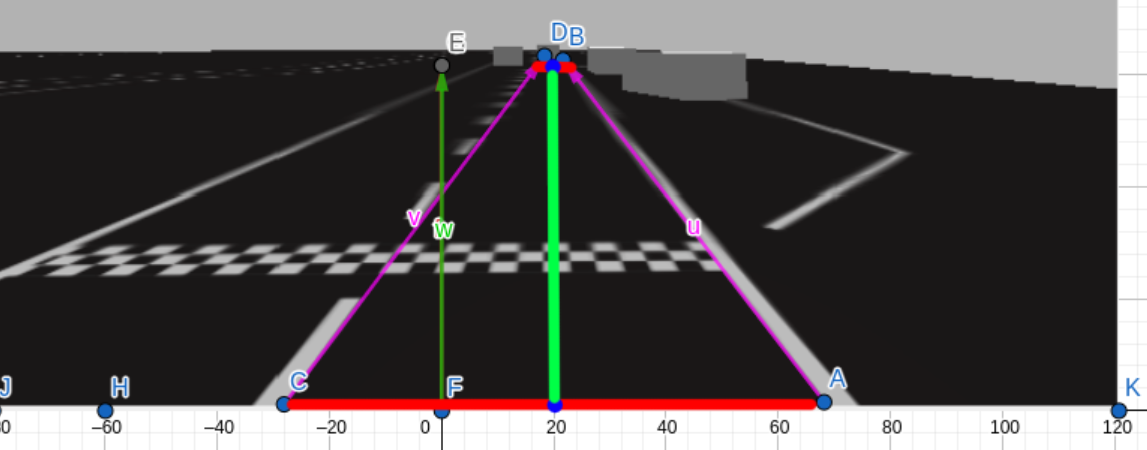
\includegraphics[width=.5\textwidth]{img/vector_gerade}
	\caption[durchschnittlichen Vektor am Start]{durchschnittlicher Vektor am Start}
	%\captionsource{So könnte man z.b. die Bildquelle angeben}
	\label{fig:vector_gerade}
\end{figure}

Diese „naive“ Idee wurde beim ersten Testen in GeoGebra bereits schnell wieder verworfen. Das Problem hierbei ist, dass wir eigentlich außerhalb von Kurven  den Vektor gespiegelt um die Y-Achse bräuchten, um zur Soll-Fahrbahn zu lenken. In den Kurven wiederum brächten wir wieder den zuvor genannten „Durchschnittsvektor“. Daher haben wir das Ganze schnell wieder verworfen, aber konnten daraus eine andere Idee entwickeln.

\begin{figure}[H]
	\centering	
	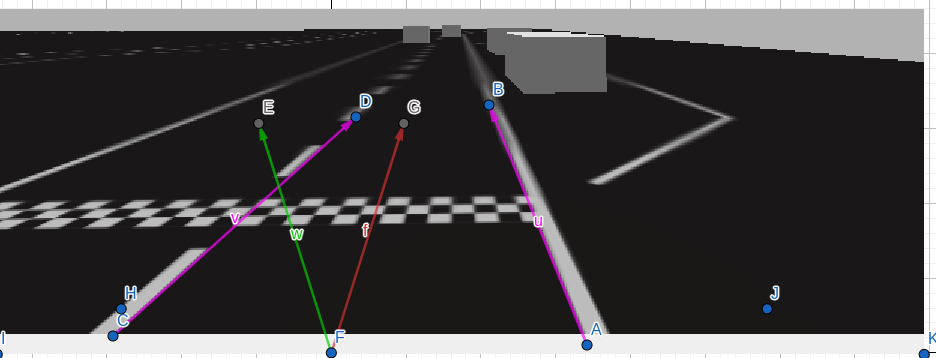
\includegraphics[width=.5\textwidth]{img/vector_zu_rechts}
	\caption[durchschnittlichen Vektor wenn zu weit rechts auf der Geraden]{durchschnittlicher Vektor wenn zu weit rechts auf der Geraden}
	%\captionsource{So könnte man z.b. die Bildquelle angeben}
	\label{fig:vector_zu_rechts}
\end{figure}

\begin{figure}[H]
	\centering	
	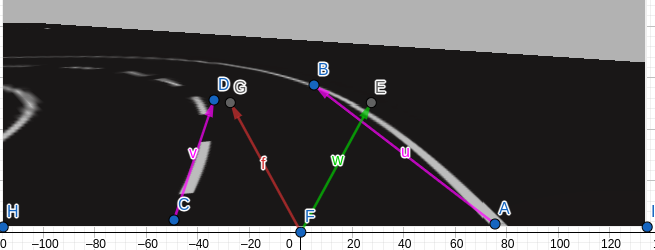
\includegraphics[width=.5\textwidth]{img/vector_kurve}
	\caption[durchschnittlicher Vektor in Kurve]{durchschnittlichen Vektor in Kurve}
	%\captionsource{So könnte man z.b. die Bildquelle angeben}
	\label{fig:vector_kurve}
\end{figure}

\begin{itemize}
			\item \color{red} Rot $\Rightarrow$ Durchschnittsvektor 	\qquad \color{green} Grün $\Rightarrow$ gespiegelter Durchschnittsvektor
			
\end{itemize}



\subsection{Weiterentwicklung der ersten Idee}
Nach Reflektieren unseres ersten Ansatzes stellen wir fest, dass uns die Y-Koordinaten eigentlich egal sein können und dass wir lediglich eine X-Koordinate benötigen, um zu wissen, ob wir nach links oder rechts lenken müssen. So kam uns die Idee, einfach den Durchschnitt aus den linken und rechten X-Koordinaten, die durch Houghline erkannt werden, zu bilden und anhand dessen die Fahrbahn zu bestimmen. Die Idee hierbei ist, die X-Koordinate der Bildmitte, die auch die Mitte des Autos ist, einfach mit der errechneten X-Koordinate zu vergleichen und anhand dessen zu lenken.

Das Ganze haben wir zunächst mit der Mittellinie und der rechten Außenlinie versucht, dabei hatten wir einige Problem mit der Mittellinie. Unter anderem das wir bei zu hoher Empfindlichkeit von Houghline zu viel Beifang hatten und bei einer zu geringen Empfindlichkeit hatten wir das Problem die Linien in den Kurven nicht mehr ausreichend zu erkennen. Darauf hin haben wir auf die beiden Außenlinien gewechselt und unsere Soll-Fahrbahn anhand der 1.25-Fachen deren Durchschnitts-X bestimmt.

Zur Bestimmung des exakten Lenkwinkels wird die X-Koordinate der Bildmitte von dem ermittelten 1.25-Fachen des Durchschnitts-X abgezogen. Das Ganze wird noch auf +- 45° abgeriegelt.

\begin{center}
$\text{Lenkwinkel} = \text{SollFahrbahn}_X - \text{Bildmitte}_X$
\end{center}


\subsection{Region-of-Interest}
Für die beiden Außenlinien gibt es je eine Region-of-Interest. Diese bekommen zunächst einen festen Startbereich. Die Region-of-Interest hatte zu Beginn bei uns eine Trapezform, die den  Linien angepasst war, durch den Perspektivenwechsel zur Top-Down-Sicht reichen nun einfache Rechtecke. Da nur der unmittelbare Bereich vor dem Auto relevant ist, wird die Höhe auch stark zugeschnitten. In den beiden Regionen nehmen wir erstmal alles, was an X-Koordinaten zu finden ist und bilden draus das zuvor genannte „Durchschnitts-X“ zum Ermitteln der Fahrbahn. Unsere Idee beim Ermitteln des Durchschnitts aus so vielen Koordinaten war, dass wenn in der Region-of-Interest Störfaktoren sind, diese einfach mit einer Überzahl an richtigen Koordinaten korrigiert wird. Sollte in einer Region-of-Interest nichts gefunden werden, wird dies bis zu einem festgelegten Maximalwert verbreitert in der Hoffnung etwas zu finden. Ist selbst bei maximaler Breite keine einzige X-Koordinate zu finden, wird einfach der letzte gefundene Wert für die entsprechende Region-of-Interest angenommen.

\begin{figure}[H]
	\centering	
	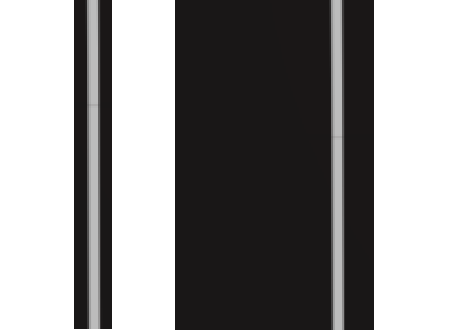
\includegraphics[width=.4\textwidth]{img/roi_breite}
	\caption[unterschiedlich Breite RoI]{unterschiedlich Breite RoI}
	%\captionsource{So könnte man z.b. die Bildquelle angeben}
	\label{fig:vector_kurve}
\end{figure}

\subsection{Verbesserung durch Top-Down-View}
Unseren Ansatz funktioniert noch deutlich besser durch einen Blick von oben. Hierfür haben wir die Kamera leicht vor dem Auto senkrecht nach unten schauend platziert. Diese vielleicht nicht ganz realistische Änderung hat zu einer solchen Verbesserung geführt, dass wir es dabei belassen haben. Eine reelle Umsetzung wäre vielleicht mit einer Drohne oder einer Art von Angel möglich, soll aber das Problem eines Maschinenbauers sein. Aus Softwareseite wäre eine Bildtransformation zu einer „pseudo“ Top-Down-Sicht möglich und sinnvoll. Zeitweise hatten wir dahin gehend auch einige Versuche unternommen, aber aufgrund von neuen Problemen, die daraus für uns entstanden sind und aus Zeitgründen haben wir es bei einer nicht so gängigen Lösung belassen.

\begin{figure}[H]
	\centering	
	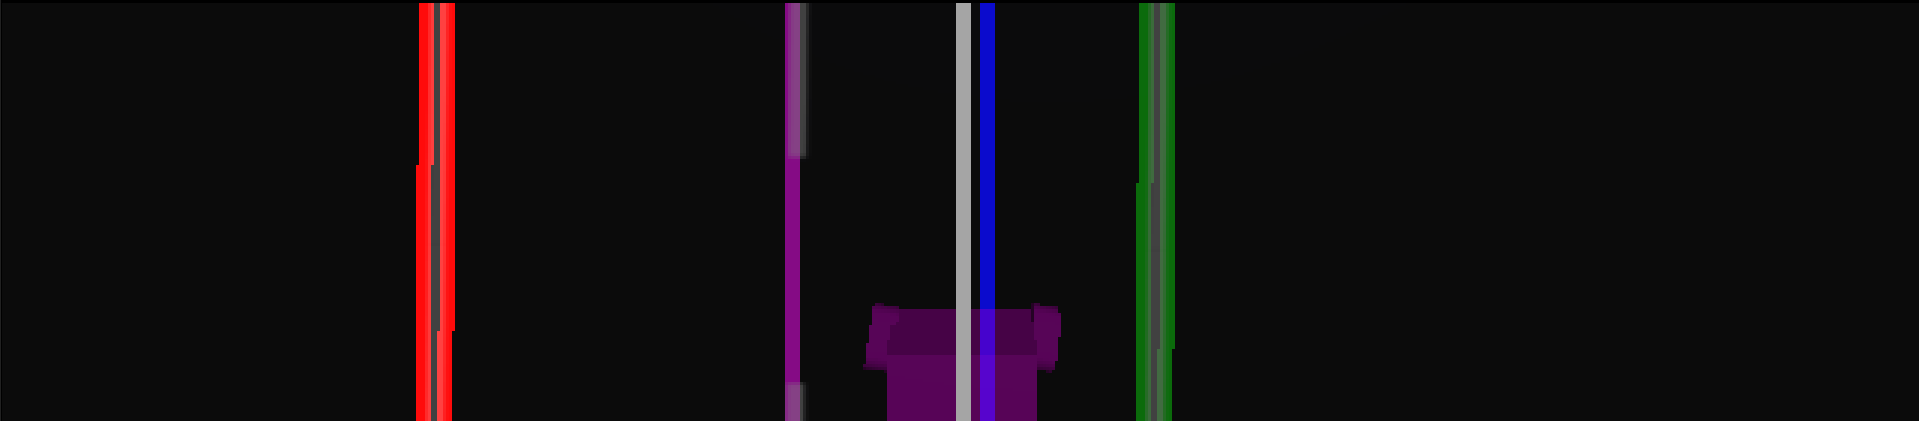
\includegraphics[width=.8\textwidth]{img/topdown _view}
	\caption[Top-Down-View]{Top-Down-View}
	%\captionsource{So könnte man z.b. die Bildquelle angeben}
	\label{fig:topdown _view}
\end{figure}

Auf der Abbildung sind die in der linienbasierten Lenkung erkannten und berechneten Linien zusehen.
\begin{itemize}
	\color{red} \item  von Houghline erkannte linke Außenlinie
	\color{green} \item  von Houghline erkannte rechte Außenlinie
	\color{violet} \item  errechnete Mittellinie = Druschnitts-X aus linken und rechten X-Koordinaten
	\color{blue} \item  1.25-Fache der Mittellinie $\Rightarrow$ Soll-Fahrbahn
	\color{gray} \item  die weiße linie ist die Bildmitte und somit auch die Automitte
\end{itemize}
Es wird angestrebt, dass die blaue und weiße Linie aufeinander liegen.

\newpage

\section{Überholmanöver}

\subsection{Verworfene Idee des \glqq blinden Mannes \glqq{}}
Ein erster Versuch das Überholmanöver zu realisieren war es das Auto rein mit dem rechten Time-of-Flight-Sensor an dem Hindernis vorbei hangeln zu lassen, ähnlich zu dem Beispiel aus der Vorlesung zum PID-Regler, bei dem es darum ging mittels eines Time-of-Flight-Sensors um eine Box im Kreis zu fahren. Bei dieser Lösung hätten wir auf die sonstigen Sensoren verzichtet und wie ein blinder Mann an ein Geländer uns an der Box entlang gehangelt. Problem für uns war bei diesem Ansatz ordentlich zuerkennen wann wir das Manöver sinnvoll beenden. Daher wurde die dahingehende Versuche auch wieder verworfen.

\subsection{Einleitung des Manövers}
Für das Überholmanöver haben wir das Fahrzeug zunächst um weitere Time-of-Flight-Sensoren ergänzt. An der Front haben wir einen sehr schmalen, nach vorne gerichteten Time-of-Flight-Sensor. Die geringe Breite ist dafür da, dass wir unnötige nicht auf der Fahrbahn befindende Boxen ignorieren. Erreicht der vordere Sensor einen gewissen Schwellenwert, überprüfen wir am linken Sensor, ob die linke Fahrbahn frei ist. Wenn dieser „Schulterblick“ sein okay gibt, wird das Überholmanöver eingeleitet.
\\
Vorbereitend wird hierbei die linienbasierte Lenkung und den Parkerknoten vorübergehend blockiert. Anschließend beginnen wir mit der ersten von fünf Phasen.

\begin{figure}[H]
	\centering	
	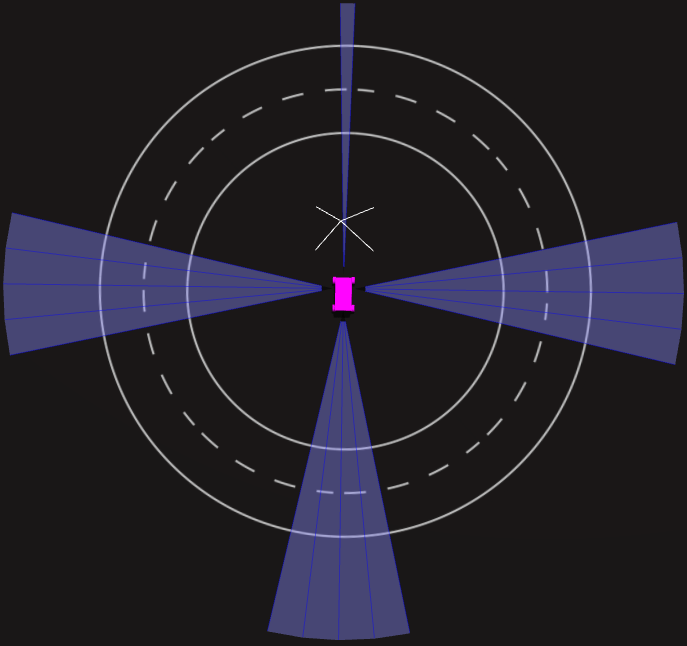
\includegraphics[width=.4\textwidth]{img/tof_sensoren}
	\caption[Verwendete ToF-Sensoren]{Verwendete ToF-Sensoren}
	%\captionsource{So könnte man z.b. die Bildquelle angeben}
	\label{fig:tof_sensoren}
\end{figure}

\subsection{5 Phasen zum Überholen}

\subsubsection{1. Phase: Spurwechsel}
Hier haben wir vereinfacht angenommen, dass man den Spurwechsel beim Überholvorgang als Gerade ansehen kann. In unserem Fall ist das ausreichend, weil das Fahrzeug nur grob auf die andere Spur kommen soll und ab da die linienbasierte Lenkung wieder ihre Aufgabe übernehmen soll. Dementsprechend kann man dann um die Überholgerade (rote Linie) ein Dreieck aufspannen. Um die gesuchte Strecke berechnen zu können, muss man nur 3 Werte kennen, was in unserem Fall die konstante effektive Spurwechseldistanz (grüne Linie), der 90°-Winkel $\gamma$ und der 25° Lenkwinkel $\beta$ sind.

\begin{figure}[H]
	\centering	
	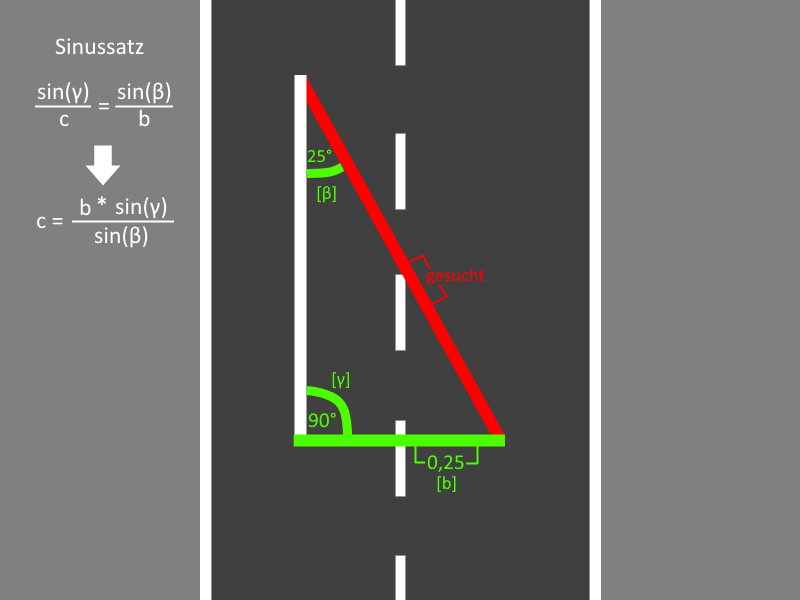
\includegraphics[width=.8\textwidth]{img/ueberholen}
	\caption[Spurwechselfahrbahn]{Spurwechselfahrbahn}
	%\captionsource{So könnte man z.b. die Bildquelle angeben}
	\label{fig:ueberholen}
\end{figure}

Über den Sinussatz wird dann einfach die Länge der Überholgeraden berechnet. Aus der zurückzulegenden Strecke und der aktuellen Geschwindigkeit wird die Dauer des Spurwechsels bestimmt. Durch Ausprobieren haben wir festgestellt, dass die berechnete Dauer konstant um den Faktor 0,9 abweicht, daher multiplizieren wir unsere errechnete Dauer noch mit 0,9. Unsere Vermutung ist, dass diese Abweichung durch die Annäherung an die tatsächlichen Überholstrecke entstanden ist.

Der ganze Aufwand ist nötig, da wir unsere Region-of-Interests nicht ohne weiteres einfach so versetzen können, diese würden bei zu frühem versetzen unter anderem die Mittellinie ungewollt erfassen, was zu einer falschen Fahrbahnbestimmung führen würde. Daher warten wir die Dauer des Spurwechsels, um dann in Phase 2 überzugehen.

\subsubsection{2. Phase: Region-of-Interest-Wechsel und warten auf Box}
Nach Ablaufen des in Phase 1 errechneten Delays, wird nun die Region-of-Interest für das Fahren auf der linken Spur angepasst. Zusätzlich muss jetzt auch unser Driveway-Factor von 1,25 zu 0,85. geändert werden. Hier würde man vermutlich 0,75 erwarten, aber durch Testen haben wir festgestellt, dass dieser Wert besser funktioniert.

Jetzt kann die linienbasierte Lenkung wieder übernehmen. Mit dem rechten Sensor warten wir darauf, die Box zu erkennen, damit wechselt das Fahrzeug dann in Phase 3.

\subsubsection{3. Phase: Warten bis die Box verschwindet}
Der Wagen ist nun auf der linken Spur und fährt an der Box vorbei. Gibt der rechte Sensor sein ok, dass die rechte Spur wieder frei ist, wechseln wir jetzt in die 4 Phase des Manövers.

\subsubsection{4. Phase: Region-of-Interest-Wechsel}
Die 4. Phase funktioniert jetzt spiegelverkehrt zur 2. Phase. Diese kümmert sich um den Wechsel der Region-of-Interest zurück auf die Startposition und das Zurücksetzen des Driveway-Factors zu 1,25. Nach Abschluss erfolgt der Wechsel in Phase 5.

\subsubsection{5. Phase: Spurwechsel}
Die 5. Phase ist nun die gespiegelte Version der 1. Phase. Diese kümmert sich jetzt abschließend um den Spurwechsel zurück nach rechts und die wieder Freigabe des Parkerknotens.



\section{Einparken}

\subsection{Erkennen einer Parklücke in 4 Phasen}

\subsubsection{1. Phase: Erkennen der ersten Box}
Zunächst wird auf der linken Seite mittels des Time-of-Flight-Sensors nach einem Erstkontakt mit einer Box geschaut. Wird eine Box erkannt, wird zunächst der Überholer-Knoten blockiert und anschließend wird in Phase 2 gewechselt.

\subsubsection{2. Phase: Erkennen der Lücke}
In der zweiten Phase wird gewartet, bis das Auto an der ersten Box vorbei ist und der linke Time-of-Flight eine Lücke erkannt hat. Ist diese erkannt, wird in die 3 Phase gewechselt.
\begin{figure}[H]
	\centering	
	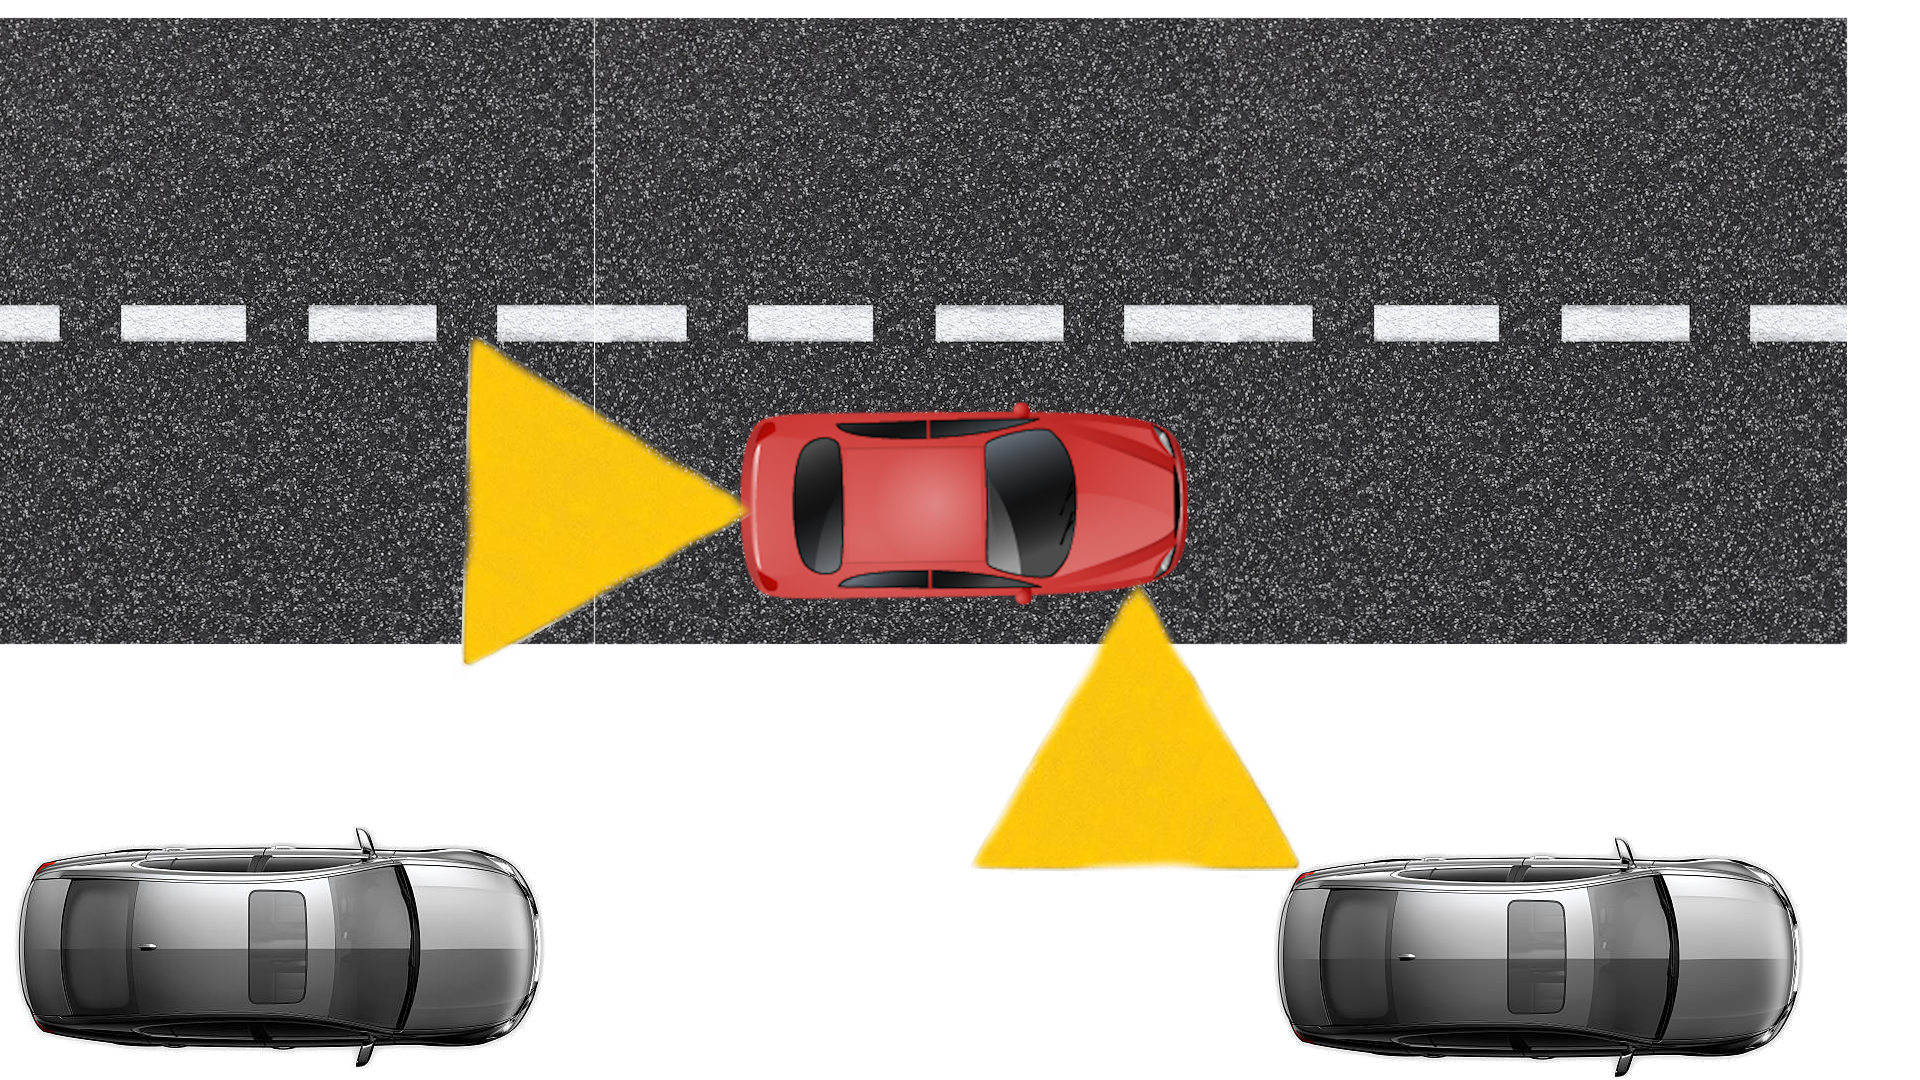
\includegraphics[width=.5\textwidth]{img/Parken}
	\caption[Parklücke erkennen]{Parklücke erkennen}
	%\captionsource{So könnte man z.b. die Bildquelle angeben}
	\label{fig:Parken}
\end{figure}

\subsubsection{3. Phase: Erkennung der zweiten Box}
Diese Phase funktioniert recht ähnlich zur 1. Phase. Es wird wieder darauf gewartet, dass auf der linken Seite eine Box erkannt wird. Ist das der Fall, wird die linienbasierte Lenkung blockiert und Phase 4 eingeleitet.



\subsubsection{4. Phase: Einleiten des Parkmanövers}
Das Auto wird hier angehalten und die Parklückenerkennung wird blockiert. Abschließend wird mit der 1. Phase des Einparkens weiter gemacht.


\subsection{Einparken}
Das Einparken ist vom Grundaufbau dem Überholen recht ähnlich und verwendet daher auch die gleichen Ansätze. Zunächst werden die Teilprobleme wieder in Phasen aufgeteilt. 

\subsubsection{1. Phase: Einfahren in die Lücke}
Sobald der Wagen die Lücke gefunden hat, fährt er noch einstück weiter Gradeaus und dann führt er einfach einen Spurwechsel im selben Schema vom Überholemanöver aus.

\subsubsection{2. Phase: Erreichen der Parkposition}
Sobald der Wagen dann in der Parklücke ist, fährt er solange rückwärts, bis der hintere ToF-Sensor anschlägt, dann bleibt der Wagen einfach kurz stehen und geht in die nächste Phase.

\subsubsection{3. Phase: Ausparken}
Hier fährt der Wagen dann einfach wieder mit einem einfachen Spurwechsel vorwärts aus der Parklücke zurück in die Fahrbahn. Es wird noch ein Timer von 20s aktiviert, der dann auch wieder den Scan freigibt, dass braucht es, da der Wagen ansonsten beim Rausfahren die zweite Box erkennen würde und in der zweiten Runde dann schon bei der ersten Box versuchen würde einzuparken.

\section{Geschwindikeitsregler}
Der Geschwindkeitsregler ist sehr simpel gehalten und ist nur außerhalb von den Manövern aktiven. In den Manövern sind feste Geschwindigkeiten. Unsere Geschwindigkeitsbestimmung basiert auf dem aktuellen Lenkwinkel, ist dieser unter einem Schwellwert, wird beschleunigt. Nach einer Wartezeit wird der Schwellenwert erneut geprüft und ggf. weiter beschleunigt, das Ganze wiederholt sich bis entweder die maximale Geschwindigkeit erreicht wurde oder der Schwellenwert überschritten ist. Ist der Schwellenwert überschritten, wird die Geschwindigkeit auf einen minimalen Wert gesetzt.


